\documentclass[titlepage,a4paper]{jsarticle}
\usepackage{../../sty/import}% 各種パッケージインポート
\usepackage{../../sty/title}% タイトルページの変更
\usepackage{otf}% ローマ数字を使えるようにするやつ
% \usepackage{svg}% SVG画像を読み込めるようにするやつ %なんかコンパイルでなんかしなきゃらしい.面倒そう
\renewcommand{\thesection}{課題\arabic{section}}
%% タイトルページの変数
% レポートタイトル
\title{マーケティング\ajRoman{2}課題まとめ}
% 提出日
\expdate{\today}
% 科目名
\subject{マーケティング\ajRoman{2}}
% 分野
\class{情報経営システム工学分野}
% 学年
\grade{B3}
% 学籍番号
\mynumber{24336488}
% 記述者
\author{本間三暉}
% グループ名 % もし班があるやつならtitle_team.styを入れる
% \team{10}
% 共同実験者 % もし共同実験者が必要なやつならtitle_kyoudou.styを入れる
% \coauthor{%
% \textbf{学籍番号:} & \textbf{氏名:} \\
% \textbf{学籍番号:} & \textbf{氏名:}\\
% \textbf{学籍番号:} & \textbf{氏名:}\\
% \textbf{学籍番号:} & \textbf{氏名:}\\
% }
%
% 記載例:
%\coauthor{%
% 学籍番号:24567321 & 氏名:吉田 富美男 \
% 学籍番号:12345678 & 氏名:安藤 雅洋 \
% 学籍番号:13579234 & 氏名:雲居 玄道 \
%%

\begin{document}
% titleページ作成
\maketitle
\section{スイッチングコストが高いと考える商品、またはサービスをひとつ選び、その概要について説明してください。}
\textbf{選択した商品・サービス:}ERPシステム(企業向けの統合基幹業務システム)

ERP(Enterprise Resource Planning)システムは,企業が経営資源を一元管理し業務の効率化を図るための統合システムである.
財務管理,人事管理,販売管理,生産管理などの機能が統合されており,企業全体で情報を共有し業務の最適化が可能となる.

ERPシステムのスイッチングコストは非常に高いとされる.
まず,金銭的コストとしては新システムのライセンス費用やハードウェアの追加導入費が発生する.
さらに,既存システムの廃棄に伴う損失も無視できない.
次に,物理的コストとしてデータ移行やシステム統合に要する時間と労力がかかる.
この過程ではデータのバックアップやシステム設定の変更が必要となるため作業負担は大きい.
心理的コストも高く,新システムの操作習得には時間と教育が求められ,従業員の抵抗感も発生し得る.
また,新しいシステムを見つけるまでに要する調査や評価にかかる探索コストも重要である\cite{slide1}.

ERPシステムは,その利便性と引き換えに高いスイッチングコストを伴うため,企業は慎重に検討し導入後の安定運用を確保することが求められる.
スイッチングコストの存在が,企業にとって大きな障壁となることは否めない\cite{slide1}.

\section{独自のポジションを獲得できていると考える商品、または企業をひとつ選び、その特徴を示すポジショニングマップを作成するときの分析軸(2軸)を選び、対象の商品(企業)の位置づけなどについて説明する。}
% ポジショニングマップを示す.
\textbf{選定企業:}アサヒビール(アサヒスーパードライ)
アサヒビールは「アサヒスーパードライ」を発売して以来,「辛口ドライビール」の市場において独自のポジションを確立している\cite{slide1}.
この製品は競合のビール会社との差別化を図りつつ市場で高い認知度を獲得している.

\subsection{分析軸}
\subsubsection{味の特徴(辛口・甘口)}
ドライビールは一般的に「辛口」とされ,キレのある飲み口が特徴である.
アサヒスーパードライは,まさにこの「辛口」を打ち出し,消費者に強い印象を与え続けている.

\subsubsection{価格(高価格・低価格)}
ビール市場においては価格も消費者の選択に大きな影響を与える.
アサヒスーパードライはプレミアムビールほど高価格ではないが,手頃な価格で提供されており大衆的な人気を保ちつつある.

\subsection{ポジショニングマップ}
この2軸でポジショニングマップを作成すると,味の特徴が「辛口」に位置し,価格が「中程度」の位置にアサヒスーパードライを置くことができる.
競合製品としてはキリンやサッポロの類似ドライビールが近い位置に存在するが,
アサヒの「元祖ドライビール」という強いブランド力が独自のポジションを保つ要因となっている.

また,比較対象としてキリンビール,サッポロビール,エビスビールを挙げる.
味の特徴と価格の2軸を取ってアサヒビール,キリンビール,サッポロビール,エビスビールを配置したポジショニングマップを図\ref{map}に示す.
\begin{figure}[H]
  \centering
  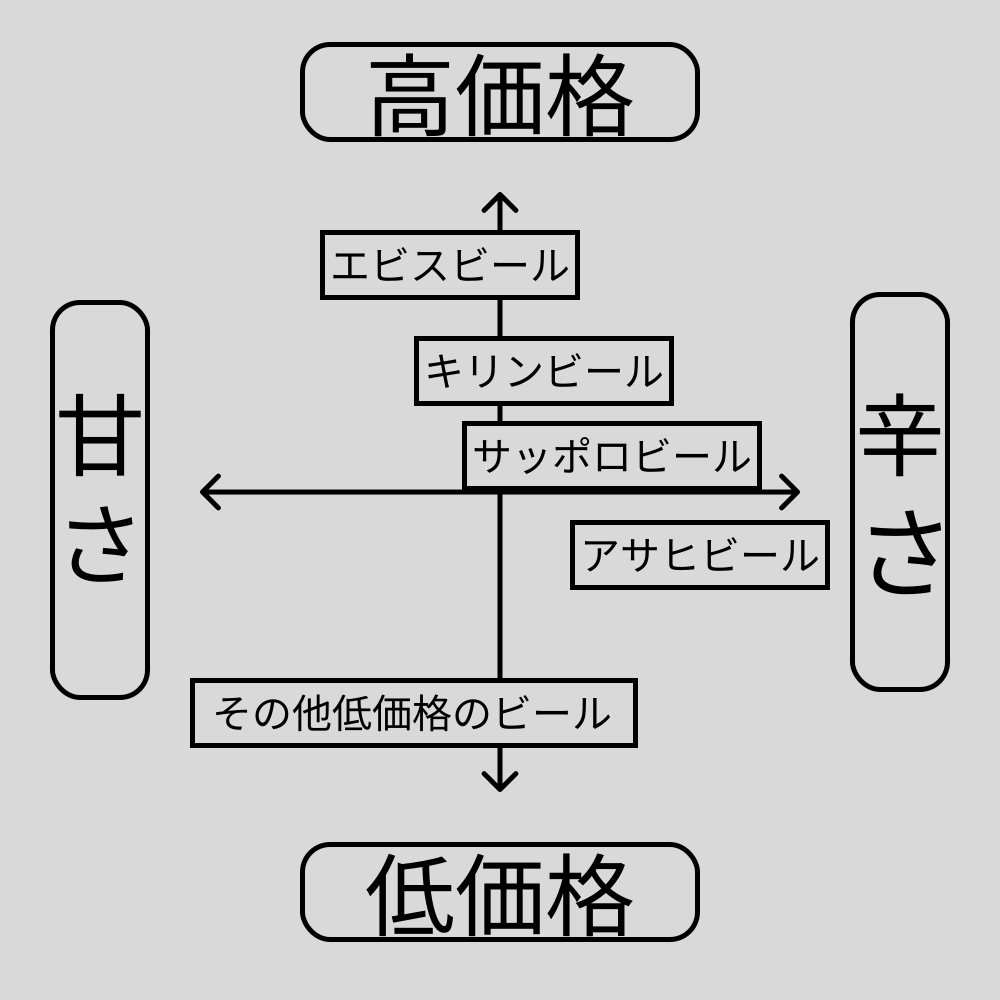
\includegraphics[width=0.8\textwidth]{img/pMap.png}
  % \includesvg
  % \includeinkscape[width=5cm]{img/pMap.svg}
  \caption{ビールに関するポジショニングマップ}
  \label{map}
\end{figure}

\subsubsection{キリンビール(キリン一番搾り)}
キリンビールは,その「一番搾り製法」を前面に押し出し,高品質なビールとしてのイメージを確立している.
キリン一番搾りは,麦汁の一番搾り部分だけを使用しており,これによって他のビールとは異なるクリアでスムーズな味わいを提供している.
この製法により,「プレミアム感」や「品質の高さ」を強調し,他社との差別化を図っている.
\\\textbf{軸1:味の特徴(辛口・甘口)}

キリン一番搾りは,アサヒスーパードライに比べてやや「甘口」であり,飲みやすさを強調している.
\\\textbf{軸2:価格(高価格・低価格)}

価格はアサヒスーパードライと同等かやや上の「中価格帯」に位置しているが,「プレミアム感」を打ち出す点で区別されている.

\subsubsection{サッポロビール(サッポロ黒ラベル)}
サッポロビールは,「サッポロ黒ラベル」を代表とする製品で,「男性的で力強いビール」というブランディングを行っている.
サッポロ黒ラベルは長年にわたり「大人のビール」としてのイメージを強く訴求しており,特に成熟した消費者層にアピールしている.
広告キャンペーンでもシンプルさと力強さを前面に出し,他のビールとは一線を画している.
\\\textbf{軸1:味の特徴(辛口・甘口)}

サッポロ黒ラベルは,「中辛口」で,バランスの取れた味わいを提供している.
アサヒスーパードライほどキレが強くはないが,キリン一番搾りよりは辛口である.
\\\textbf{軸2:価格(高価格・低価格)}

サッポロ黒ラベルはアサヒスーパードライやキリン一番搾りと同様に「中価格帯」に位置しており,大衆向けながらも品質を重視したビールである.

\subsubsection{エビスビール(プレミアムビール)}
エビスビールは,サッポロビールのプレミアムブランドとして,高級感を前面に押し出している.
特に素材や製法にこだわったビールとして,「贅沢さ」や「上質さ」を強調しプレミアムビール市場において確固たる地位を築いている.
\\\textbf{軸1:味の特徴(辛口・甘口)}

エビスビールは「やや甘口」で,リッチでまろやかな味わいを提供する.
\\\textbf{軸2:価格(高価格・低価格)}

エビスビールは「高価格帯」に位置し,特に特別なシーンや贈答用として消費者に選ばれている.

\section{日本にあるコンビニで販売されている弁当の年間売上高を推計してください。}
コンビニ弁当の年間売上高を推計するには,大手3社(セブンイレブン,ローソン,ファミリーマート)のデータをもとに考える必要がある.
\subsection{セブンイレブン}
セブンイレブンは2023年に約5.1兆円の売上高を記録しており,そのうち日配食品(弁当などの短期消費品)の割合は約12.5\%である\cite{711}.
この割合をもとに,弁当などの売上は約6375億円と推定される.

\subsection{ローソン}
ローソンの全体の売上高は約2.5兆円で,同じく日配食品の売上が占める割合が大きい.
仮に同様に12.5\%と仮定すると,ローソンにおける弁当などの売上は約3125億円と推定できる\cite{Lowson}.

\subsection{ファミリーマート}
ファミリーマートは売上高が約3兆円で,こちらも同様に日配食品が12.5\%と仮定すれば,弁当売上は約3750億円となる\cite{fam}.

\subsection{推定結果}
以上を総合すると,セブンイレブン,ローソン,ファミリーマートの弁当の年間売上高は,合計で約1.32兆円と推定される.
これに他の小規模コンビニチェーンの売上が加わることを考えると,日本のコンビニ全体での弁当の年間売上はおよそ1.5兆円前後になると考えられる.

\section{企業(業種などは任意)のマーケティングにとって有効なデータを選び、IoTデバイスを用いたデータの収集方法を検討し、説明する。}
企業のマーケティングにおいて有効なデータとして\textbf{消費者行動データ}を選定する.
消費者行動データは購買傾向や来店頻度,興味・関心の商品カテゴリを把握するのに有効である.
このデータを用いることで,マーケティング戦略の最適化が可能となりプロモーションの効果を最大化するためのターゲティング精度が向上する.

\subsection*{IoTデバイスを用いたデータ収集方法:}
\subsection{スマートフォン連携センサー}
IoTデバイスとして店舗内に配置されたセンサーが,スマートフォンと連携することで来店客の行動データを収集できる.
例えば,Wi-FiやBluetoothを利用して顧客がどの棚に長く滞在していたか,どの商品の前で足を止めたかを把握する.
この情報を基に,店内レイアウトの最適化やプロモーション展開のタイミングを調整できる.

\subsection{スマートシェルフ}
スマートシェルフは商品の在庫や売れ行きのデータをリアルタイムで記録し,消費者がどの商品を手に取ったか,または戻したかなどの詳細なデータを収集できる.
これにより,特定商品の売上状況だけでなく消費者の関心度を高める商品の配置方法を改善できる.

\subsection{ウェアラブルデバイス}
特定の業種では顧客にウェアラブルデバイスを提供し,心拍数や移動パターンを分析することで商品の購買意欲を高める環境づくりに役立てることができる.
例えば,フィットネスクラブなどでは顧客の運動データを基にした商品やサービスの提案が可能となる.

\subsection{まとめ}
これらのIoTデバイスを活用したデータ収集により,リアルタイムで消費者の行動を把握しマーケティング戦略を強化できると考える.


% \section{ひとつのモノ(商品・サービス)を任意で選び、選定した モノとそれと競合するモノをひとつ以上選んだうえで、それぞれを分類するマトリクスを作成する。
%   マトリクスの作成においては、モノの特徴を考慮し、縦軸の上下、横軸の左右、それぞの分析軸を示す。
%   選んだモノ、および競合するモノをプロットしたうえで、それぞれの特徴をターゲットとともに説明してください。}




% 参考文献
\begin{thebibliography}{99}
  \bibitem{slide1} 令和6年 マーケティング\ajRoman{2}授業スライド
  \bibitem{711} セブンイレブンの公式データ\url{https://www.sej.co.jp/company/yokogao/data/}
  \bibitem{Lowson} ローソンIR資料\url{https://www.lawson.co.jp/company/ir/library/annual_report/2022/pdf/ar2022_P64-67.pdf}
  \bibitem{fam} ファミリーマートの分析記事\url{https://smbiz.asahi.com/article/14601977}
\end{thebibliography}

\end{document}